\chapter{Methodology and Study Design} \label{chapter::study_design}
This chapter explores the employed methodology for testing both the performance hypothesis $H_P$ and the usability hypothesis $H_U$ (defined in Section \ref{section::thesis_objective}). 
The goal is to explicitly show the reasoning for the chosen methods as well as provide specific method implementation details to aid transparancy about the obtained results discussed in Chapter \ref{chapter::results}.\\
Generally, the employed methodology to achieve the research objective (Section \ref{section::thesis_objective}) is to replicate a relevant subset of functionality of an existing iOS app using Flutter. Thereby, the \textbf{original app} acts as a baseline with which the \textbf{Flutter clone} 
can be comparatively evaluated. Based in this comparison, the research question - whether the Flutter framework can match native performance and provide equivalent usability (Section \ref{section::thesis_objective}) - is answered.
Instead of creating artificial use cases, taking advantage of an existing app provides realistic instances for performance as well as user interface testing.\\
The first section in this chapter (Section \ref{section::facet_selection}) details the decision process for selecting the baseline testing app as well as its feature reduction for further comparison. 
The subsequent two sections (Sections \ref{section::performance_comparison_design} and \ref{section::usability_comparison_design}) explore the specific methods and reasoning for the performance and 
usability comparison respectively.




\section{Baseline App Selection Process} \label{section::facet_selection}
The procedure for choosing the case study app is based on a 4 step filtering process. Each step may be viewed as a constraint
applied upon possible apps progressively reducing the number of potential baseline testing apps:
\begin{enumerate}
    \item The app is built and maintained by apploft. \label{item::constraint_one}
    \item The app includes common application \textbf{facets}. \label{item::constraint_two}
    \item The app uses modern iOS framework technologies. \label{item::constraint_three}
    \item The app conforms to the human interface guidelines (HIG) by Apple (\cite{Apple2021a}). \label{item::constraint_four}
\end{enumerate}
The reasoning behind selecting the above filtering constraints is detailed in the following paragraphs.

\subsection*{Creation and Maintainance by apploft}
This constraint was imposed on the filtering process such that a contact person (apploft
employee) is available for code specific questions.\\
Having a reference to the original source code further provides the ability of implementing the Flutter replica similarly to facilitate comparability with the baseline app.
E.g. a particular algorithm could be implemented similarly in the Flutter application. Thereby, equivalent time and space complexities are produced and 
algorithm implementation can be retracted as a confounding variable.\\
Furthermore, access to the original source code provides the ability to reduce unnecessary features which are irrevalent regarding the hypotheses evaluation. This reduces the complexity of the Flutter replica.

\subsection*{Inclusion of Common Application Features}
The goal of this thesis is to determine whether Flutter is comparable in terms of performance ($H_P$) and usability ($H_U$) for the archetypal mobile app (Section \ref{section::methods}). 
Therefore, only facets commonly appearing in iOS apps are considered for finding the baseline testing app.\\
For the purposes of finding the baseline app, a \textbf{facet} is defined as either
\begin{enumerate}[label=(\alph*)]
    \item a generalizable UI component which is non-trivial, or \label{item::facet_ui}
    \item an underlying technical attribute influencing the user experience. \label{item::technical_attribute}
\end{enumerate}

Trivial UI components \ref{item::facet_ui} such as buttons or text weren't considered \textbf{facets} as they are omnipresent throughout every app.
As for \ref{item::technical_attribute}, a technical attribute has to influence the user experience to be incorporated as the purpose of this thesis is testing Flutter's value as a UI framework (see Section \ref{section::thesis_objective}).
For example, networking can be viewed as a \textbf{facet} if fetched data is displayed via the UI, but is not a \textbf{facet} if the sole purpose of networking within 
an app is to extract analytics data.

\subsection*{Use of Modern iOS Frameworks}
If this constraint were not applied on the filtering process, old iOS technology could be compared to a modernly built Flutter app. 
Therefore, constraining the baseline app to be built with modern iterations of iOS framework technology ensures a reasonable comparison 
against the replica app.

\subsection*{Conformance to Human Interface Guideline}
Conforming to Apple's HIG ensures the original app looks native to the iOS platform.
Since Flutter comes from Google, it probably implements the \textbf{Material Design} (\cite{Google2021}) rather well. Rebuilding an app that conforms to Apple's design guidelines is the more interesting case.\\
In addition, providing a recognizable UX for iOS users would keep participants in the usability study (detailed in Section \ref{section::usability_comparison_design}) focused on noticing differences instead of 
being distracted by an ambiguous UI.
\hfill \break

Based on the above constraints, a small study was conducted looking at 15 apps developed by apploft (constraint \ref{item::constraint_one}) from 9 different iOS App Store categories. 
The factes were extracted into Table \ref{tab::initial_table} by going through each user interface (constraint \ref{item::constraint_two}).
Furthermore, a facet had to appear at least twice before being added as a result.\\
Continuing the filtering process, as per constraint 2 uncommon facets - facets appearing
in less than 50\% of observed apps - are excluded. This reduces the list of facets to the following:

\begin{itemize}
    \item \textbf{Networking} - Interaction with a remote API.
    \item \textbf{Login/Authentication} - User log in meachanism through a UI.
    \item \textbf{Tab navigation} - UI component to quickly switch between different sections of an app (\cite{AppleHIGTabBar2021}).
    \item \textbf{Hierarchical navigation} - Screens opened on top of previous screens using a stack structure (\cite{AppleHIGNavigation2021}).
    \item \textbf{Keyboard interaction} - UI for inputing text via a software keyboard.
    \item \textbf{Vertically scrolling collections} - UI collection of items scrolling vertically.
    \item \textbf{Horizontally scrolling collections} - UI collection of items scrolling horizontally.
    \item \textbf{Webview component integration} - Integrated UI component for displaying web content (\cite{AppleHIGWebViews2021}).
\end{itemize}

Out of the 15 initially tested apps, 5 include all of the above \textbf{facets} (conforming to
constraint 1 and 2) (see Table \ref{tab::filtered_table}). Kickdown (see Section \ref{section:kickdown_feature_presentation}) is chosen among the remaining 
contestants for the baseline testing app. It was most recently released (Feb 2021) and is therefore built with modern iOS technologies (constraint \ref{item::constraint_three})
and complies to the most recent iteration of the \textbf{Human Interface Guidelines} (constraint \ref{item::constraint_four}).

\subsection{Clone Application Feature Reduction and Implementation} \label{subsection::clone_app_feature_reduction}
The login and signup mechanism - although a common \textbf{facet} - is removed from the original
app for baseline testing. This is due to the fact that textfield and button interaction as well
as networking is already present in other parts of the app and would yield no further insight
regarding the hypotheses evaluation.\\
The Flutter app is implemented as closely as possible to the original application to avoid an
asymmetrical comparison as detailed in Chapter \ref{chapter::implementation}.

\afterpage{
    \clearpage
    \thispagestyle{empty}
    \begin{landscape}
        \begin{center}
            \begin{table}[!htp]
                \caption{Initial Facet Extraction for apploft's Apps}\label{tab::initial_table}
                \tiny
                \begin{tabular}{lrrrrrrrrrrrr}\toprule
                \textbf{} & & &\cellcolor[HTML]{A8A8A8}\textbf{Login/} & &\cellcolor[HTML]{A8A8A8}\textbf{Tab} &\cellcolor[HTML]{A8A8A8}\textbf{Stack} &\cellcolor[HTML]{A8A8A8}\textbf{Keyboard} &\cellcolor[HTML]{A8A8A8}\textbf{Vertically Scrolling} &\cellcolor[HTML]{A8A8A8}\textbf{Horizontally Scrolling} &\textbf{Webview} &\textbf{Camera} \\
                \textbf{App} &\textbf{category} &\cellcolor[HTML]{A8A8A8}\textbf{Networking} &\cellcolor[HTML]{A8A8A8}\textbf{Authentication} &\textbf{Maps} &\cellcolor[HTML]{A8A8A8}\textbf{Navigation} &\cellcolor[HTML]{A8A8A8}\textbf{Navigation} &\cellcolor[HTML]{A8A8A8}\textbf{Interaction} &\cellcolor[HTML]{A8A8A8}\textbf{Collection} &\cellcolor[HTML]{A8A8A8}\textbf{Collection} &\textbf{Components} &\textbf{Interaction} \\\midrule
                bonprix &shopping &1 &1 & &1 &1 &1 &1 &1 &1 & \\
                couponplatz &shopping &1 &1 &1 &1 &1 &1 &1 &1 &1 & \\
                Fernsehlotterie &lifestyle &1 & & &1 &1 &1 &1 &1 &1 & \\
                Gerolsteiner TrinkCheck &health & & &1 & &1 & &1 & &1 & \\
                Hexal Pollenflug &weather &1 & & &1 &1 &1 &1 & &1 & \\
                HIPP Baby &health &1 &1 &1 &1 &1 &1 &1 & &1 &1 \\
                Hipp Bio &food &1 & & & &1 & &1 & &1 &1 \\
                Hipp Buddies app &family & & & & &1 & &1 &1 & & \\
                Hipp Windel &shopping &1 & & &1 &1 & &1 &1 &1 &1 \\
                Kickdown &shopping &1 &1 & &1 &1 &1 &1 &1 &1 & \\
                Lotto Nds. &entertainment &1 &1 & &1 &1 &1 &1 &1 &1 & \\
                Kulturpunkte &travel &1 & &1 & &1 & &1 & & & \\
                Servus TV &entertainment &1 &1 & &1 &1 &1 &1 &1 &1 & \\
                Starcook &food &1 &1 & & &1 &1 &1 &1 &1 &1 \\
                Zeit Online &news &1 &1 & & &1 &1 &1 & &1 & \\
                \midrule
                &9 &\cellcolor[HTML]{A8A8A8}\textbf{13} &\cellcolor[HTML]{A8A8A8}\textbf{8} &\textbf{4} &\cellcolor[HTML]{A8A8A8}\textbf{9} &\cellcolor[HTML]{A8A8A8}\textbf{15} &\cellcolor[HTML]{A8A8A8}\textbf{10} &\cellcolor[HTML]{A8A8A8}\textbf{15} &\cellcolor[HTML]{A8A8A8}\textbf{9} &\cellcolor[HTML]{A8A8A8}\textbf{13} &4 \\
                \bottomrule
                \end{tabular}
            \end{table}
            
            \begin{table}[!htp]
                \caption{Table \ref{tab::initial_table} After Applying Constraint 2}\label{tab::filtered_table}
                \tiny
                \begin{tabular}{lrrrrrrrrrr}\toprule
                \textbf{} & & &\textbf{Login/} &\textbf{Tab} &\textbf{Stack} &\textbf{Vertically Scrolling} &\textbf{Horizontally Scrolling} &\textbf{Webview} & \\
                \textbf{App} &\textbf{category} &\textbf{Networking} &\textbf{Authentication} &\textbf{Navigation} &\textbf{Navigation} &\textbf{Collection} &\textbf{Collection} &\textbf{Components} & \\\midrule
                \cellcolor[HTML]{A8A8A8}\textbf{bonprix} &shopping &1 &1 &1 &1 &1 &1 &1 &\cellcolor[HTML]{A8A8A8}\textbf{7} \\
                \cellcolor[HTML]{A8A8A8}\textbf{couponplatz} &shopping &1 &1 &1 &1 &1 &1 &1 &\cellcolor[HTML]{A8A8A8}\textbf{7} \\
                Fernsehlotterie &lifestyle &1 & &1 &1 &1 &1 &1 &6 \\
                Gerolsteiner TrinkCheck &health & & & &1 &1 & &1 &3 \\
                Hexal Pollenflug &weather &1 & &1 &1 &1 & &1 &5 \\
                HIPP Baby &health &1 &1 &1 &1 &1 & &1 &6 \\
                Hipp Bio &food &1 & & &1 &1 & &1 &4 \\
                Hipp Buddies app &family & & & &1 &1 &1 & &3 \\
                Hipp Windel &shopping &1 & &1 &1 &1 &1 &1 &6 \\
                \cellcolor[HTML]{A8A8A8}\textbf{Kickdown} &shopping &1 &1 &1 &1 &1 &1 &1 &\cellcolor[HTML]{A8A8A8}\textbf{7} \\
                \cellcolor[HTML]{A8A8A8}\textbf{Lotto Nds.} &entertainment &1 &1 &1 &1 &1 &1 &1 &\cellcolor[HTML]{A8A8A8}\textbf{7} \\
                Kulturpunkte &travel &1 & & &1 &1 & & &3 \\
                \cellcolor[HTML]{A8A8A8}\textbf{Servus TV} &entertainment &1 &1 &1 &1 &1 &1 &1 &\cellcolor[HTML]{A8A8A8}\textbf{7} \\
                Starcook &food &1 &1 & &1 &1 &1 &1 &6 \\
                Zeit Online &news &1 &1 & &1 &1 & &1 &5 \\
                \bottomrule
                \end{tabular}
            \end{table}


        \end{center}
    \end{landscape}
}

\subsection{Kickdown App Feature Presentation} \label{section:kickdown_feature_presentation}
\textit{Kickdown} is an online auctioning platform for buying and selling classic and vintag cars (\cite{Kickdown2021}).\\
The original iOS app was built by apploft based on a subset of functionality from the web application and its underlying internal API.
The application is divided into two main sections via tab navigation: the overview and the more screen (see Figure \ref{fig:kickdown_overview_screen} and \ref{fig:kickdown_more_screen}).\\
On the overview, the user has the ability to scroll through all current offerings. Each offering is shown as a card with a hero image 
and some basic information including the title, location, current price and remaining time.\\
Tapping on a posting card brings up a detail view (Figure \ref{fig:kickdown_detail_screen}) for the respective posting.
Besides inspecting detailed information about the particular posting, the user has the option of viewing additional photos in the image gallery (Figure \ref{fig:kickdown_gallery_view}) and placing a bid via a bottom sheet (Figure \ref{fig:kickdown_bid_preparation_screen}).\\
The More screen lets the user login, turn on analytics tracking or open informational web views.

\begin{figure}[htbp]
    \begin{tabular}{p{0.33\textwidth}p{0.33\textwidth}p{0.33\textwidth}}
        \begin{minipage}{.33\textwidth}
            \centering
            \fbox{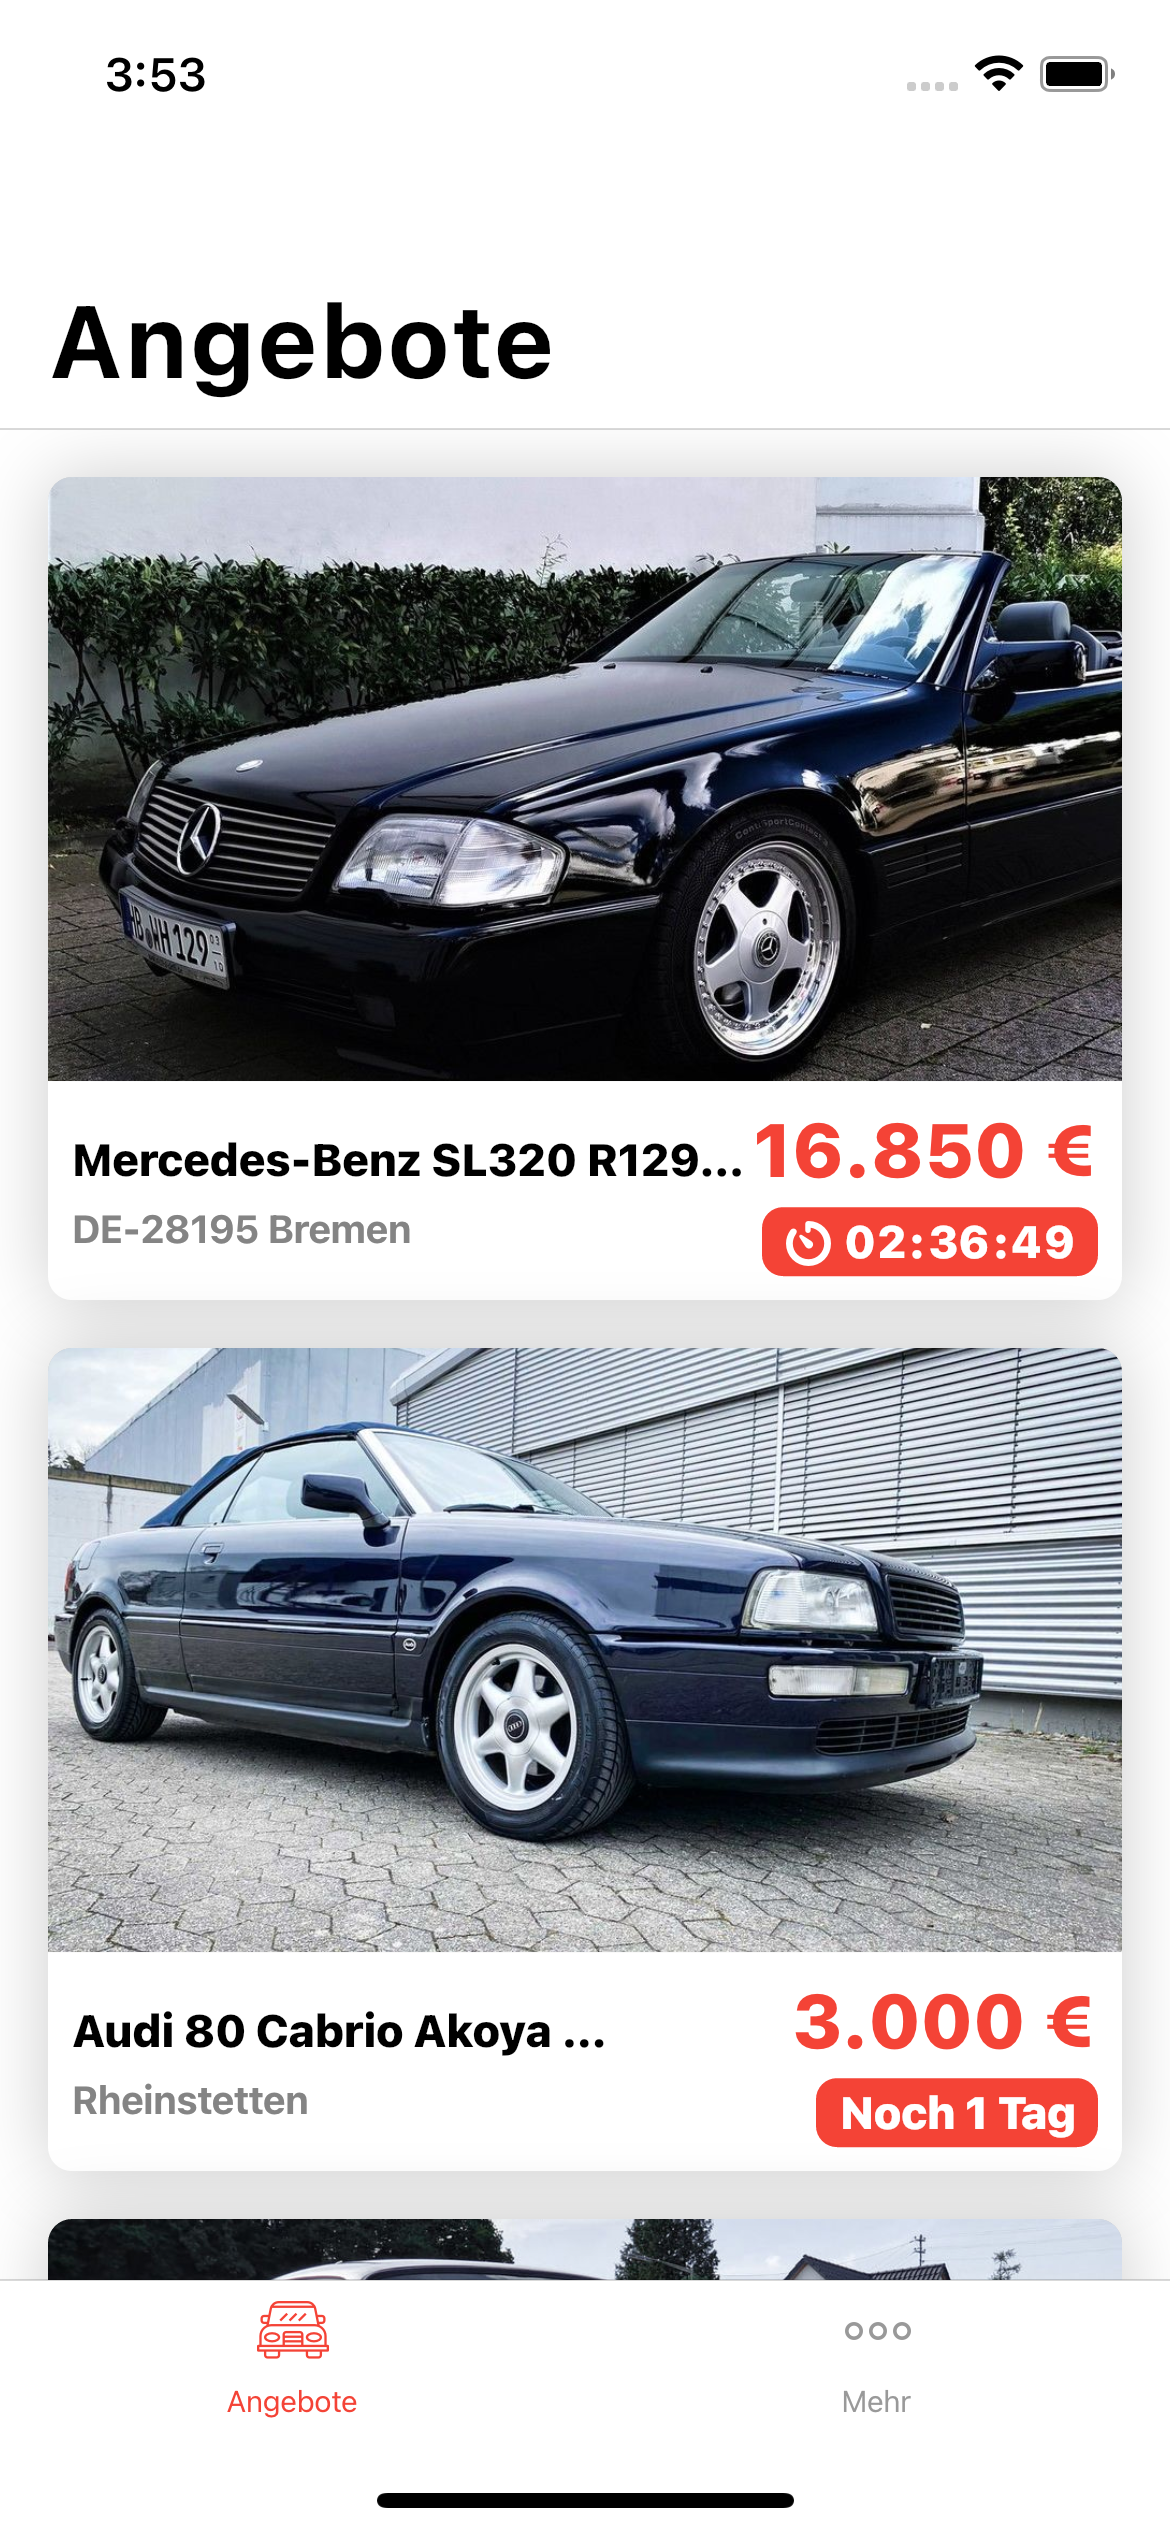
\includegraphics[width=\linewidth, height=300pt]{images/kickdown_presentation/kickdown_overview_screen.png}}
            \caption{Kickdown Postings Overview}
            \label{fig:kickdown_overview_screen}
        \end{minipage}
        &
        \begin{minipage}{.33\textwidth}
            \centering
            \fbox{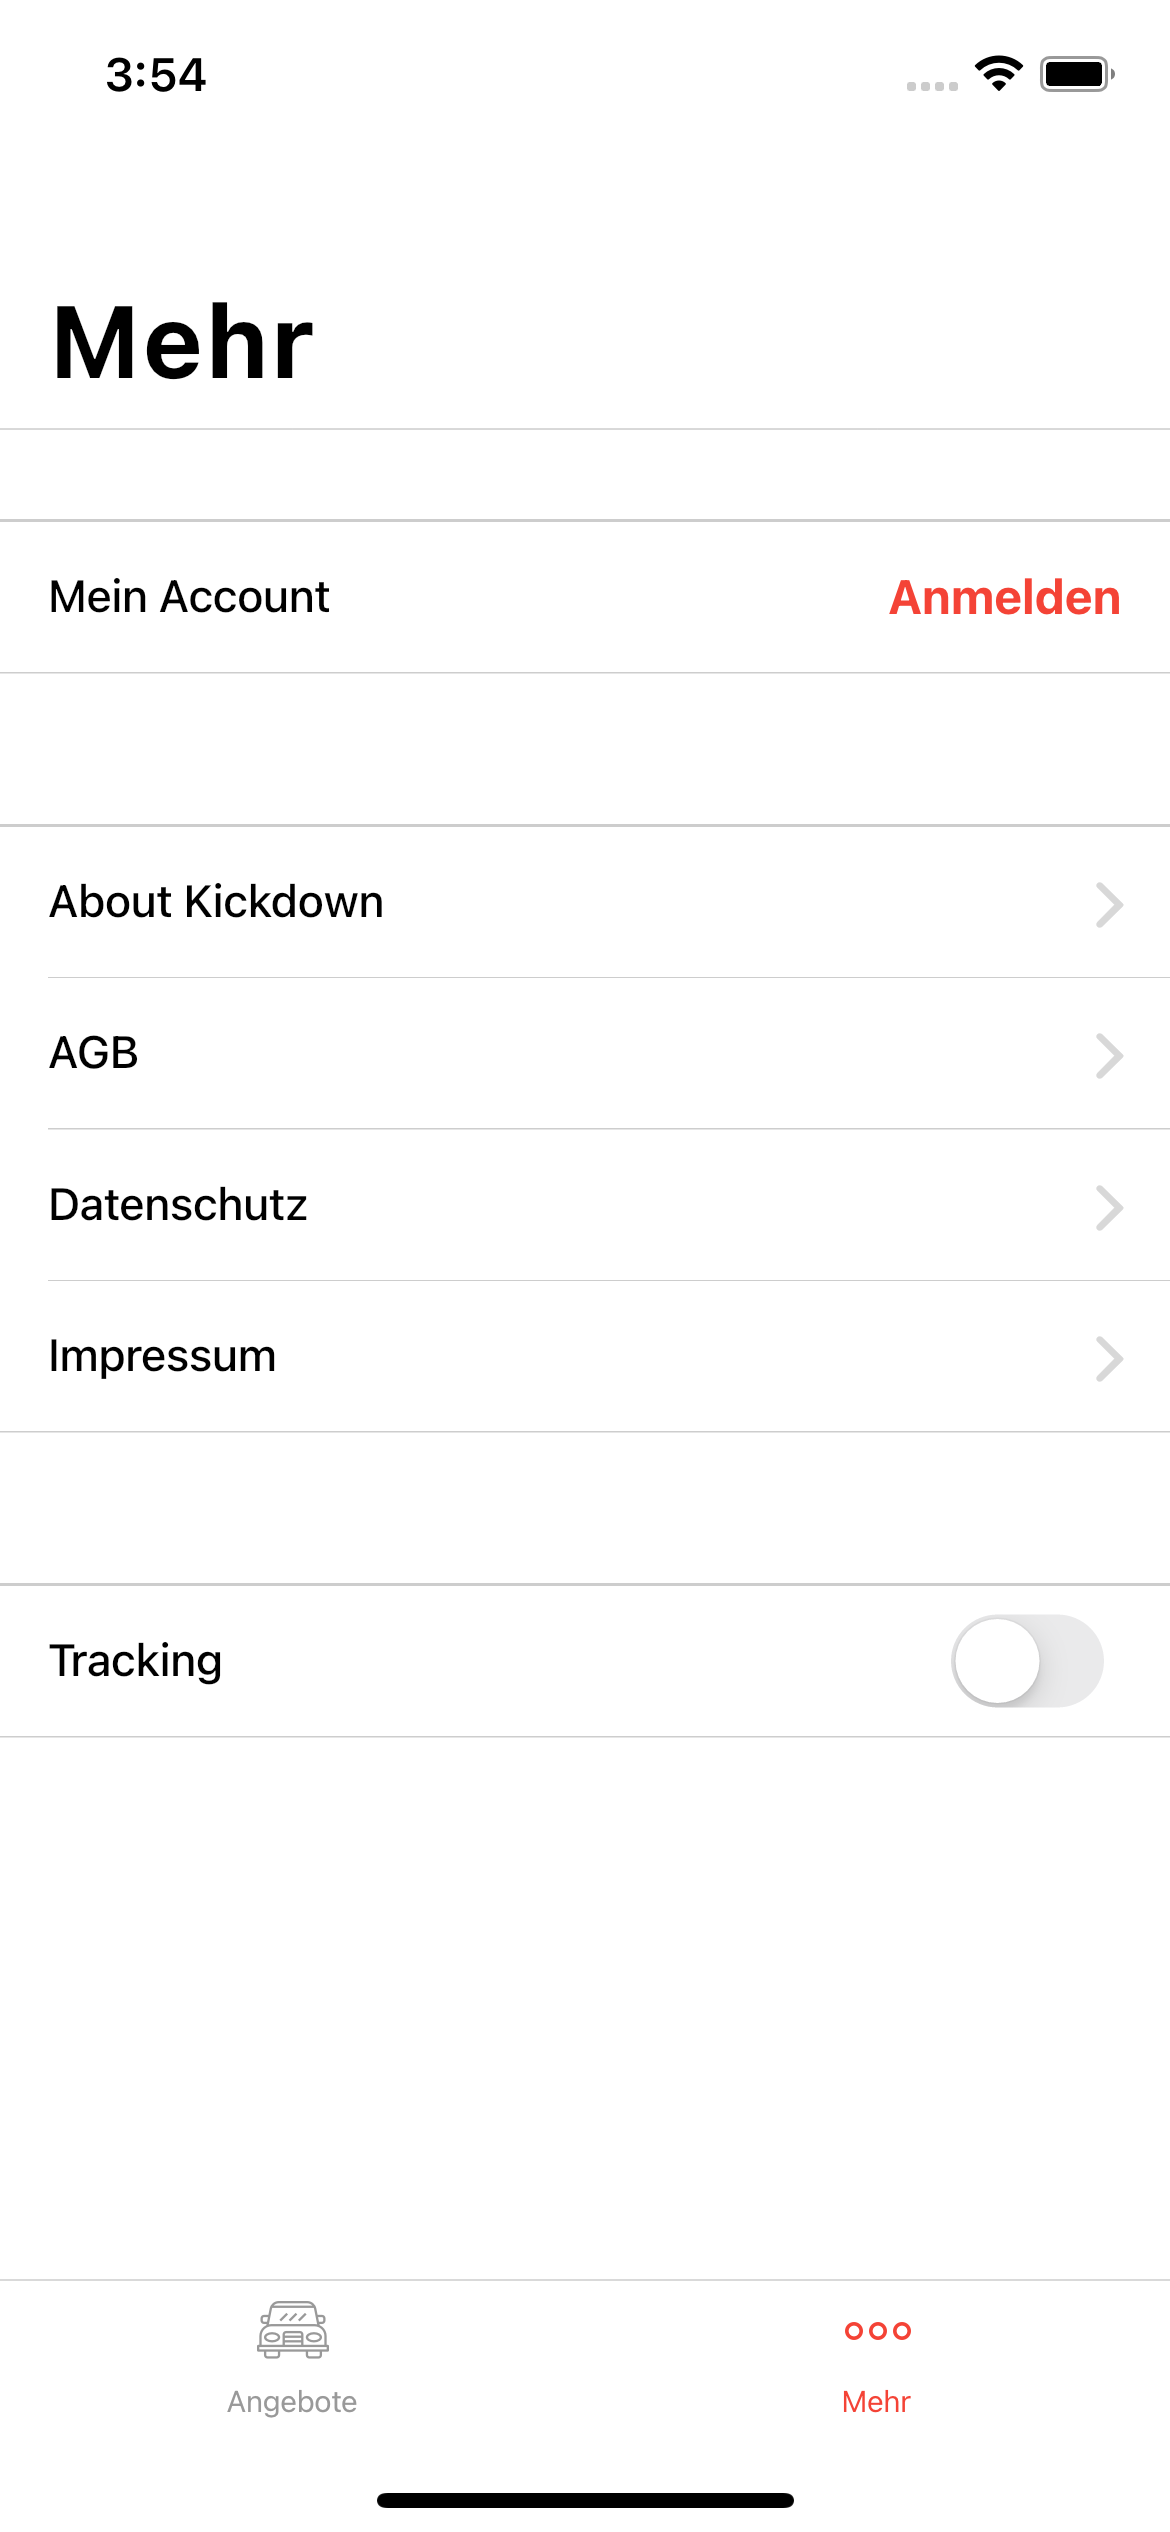
\includegraphics[width=\linewidth, height=300pt]{images/kickdown_presentation/kickdown_more_screen.png}}
            \caption{Kickdown More Screen}
            \label{fig:kickdown_more_screen}
        \end{minipage}
        &
        \begin{minipage}{.33\textwidth}
            \centering
            \fbox{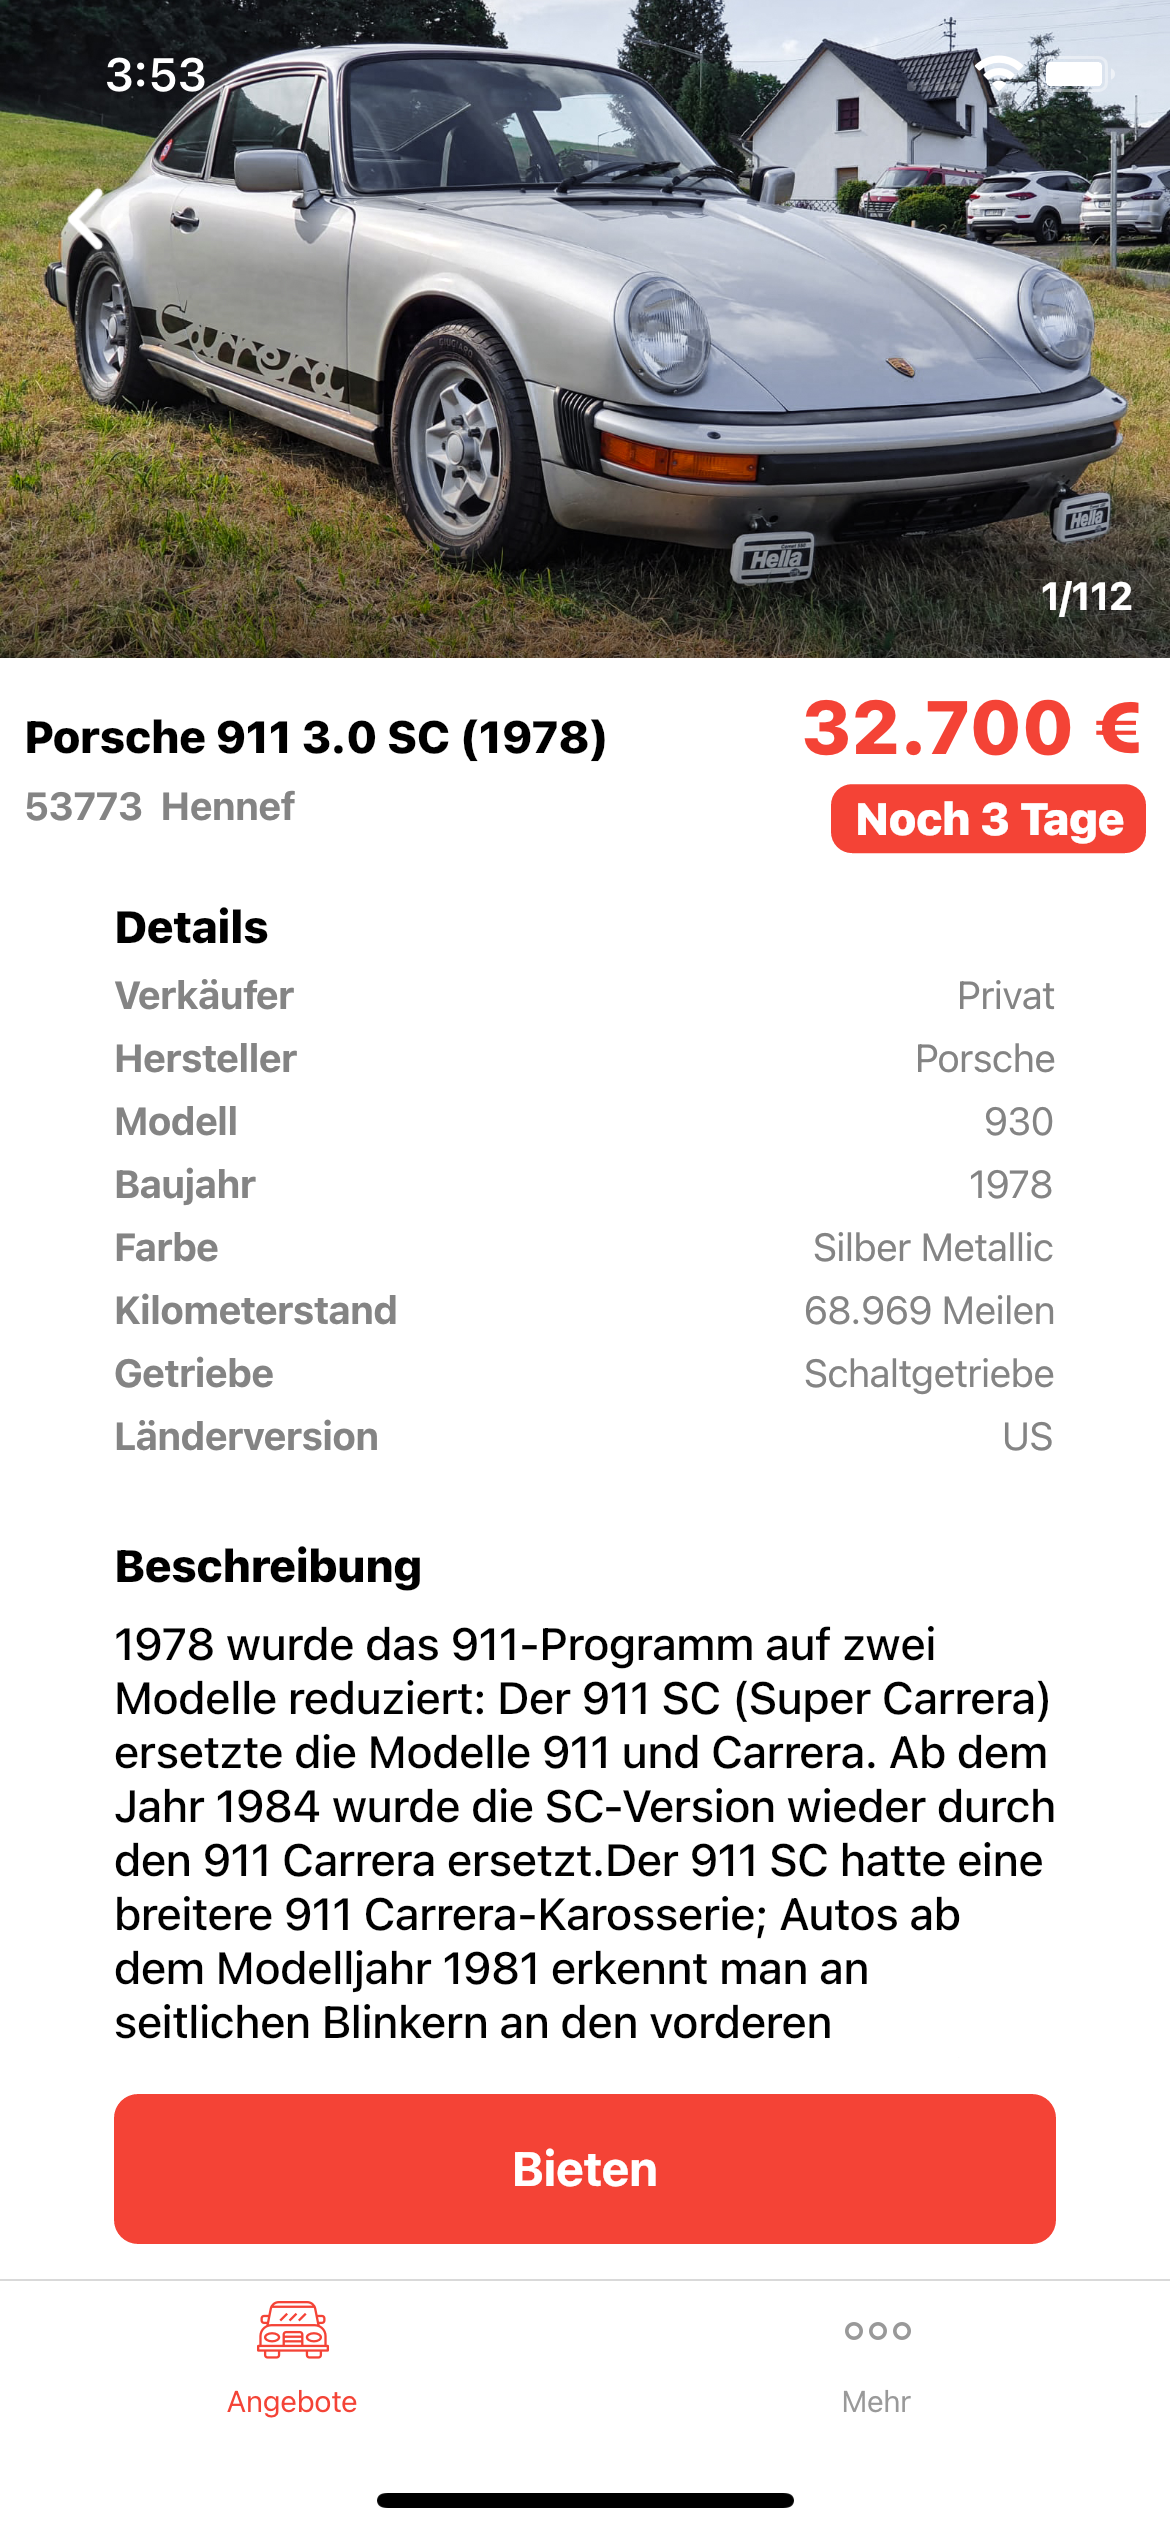
\includegraphics[width=\linewidth, height=300pt]{images/kickdown_presentation/kickdown_detail_screen.png}}
            \caption{Kickdown Detail Screen}
            \label{fig:kickdown_detail_screen}
        \end{minipage}
    \end{tabular}
\end{figure}

\begin{figure}[htbp]
    \begin{tabular}{p{0.33\textwidth}p{0.33\textwidth}p{0.33\textwidth}}
        \begin{minipage}{.33\textwidth}
            \centering
            \fbox{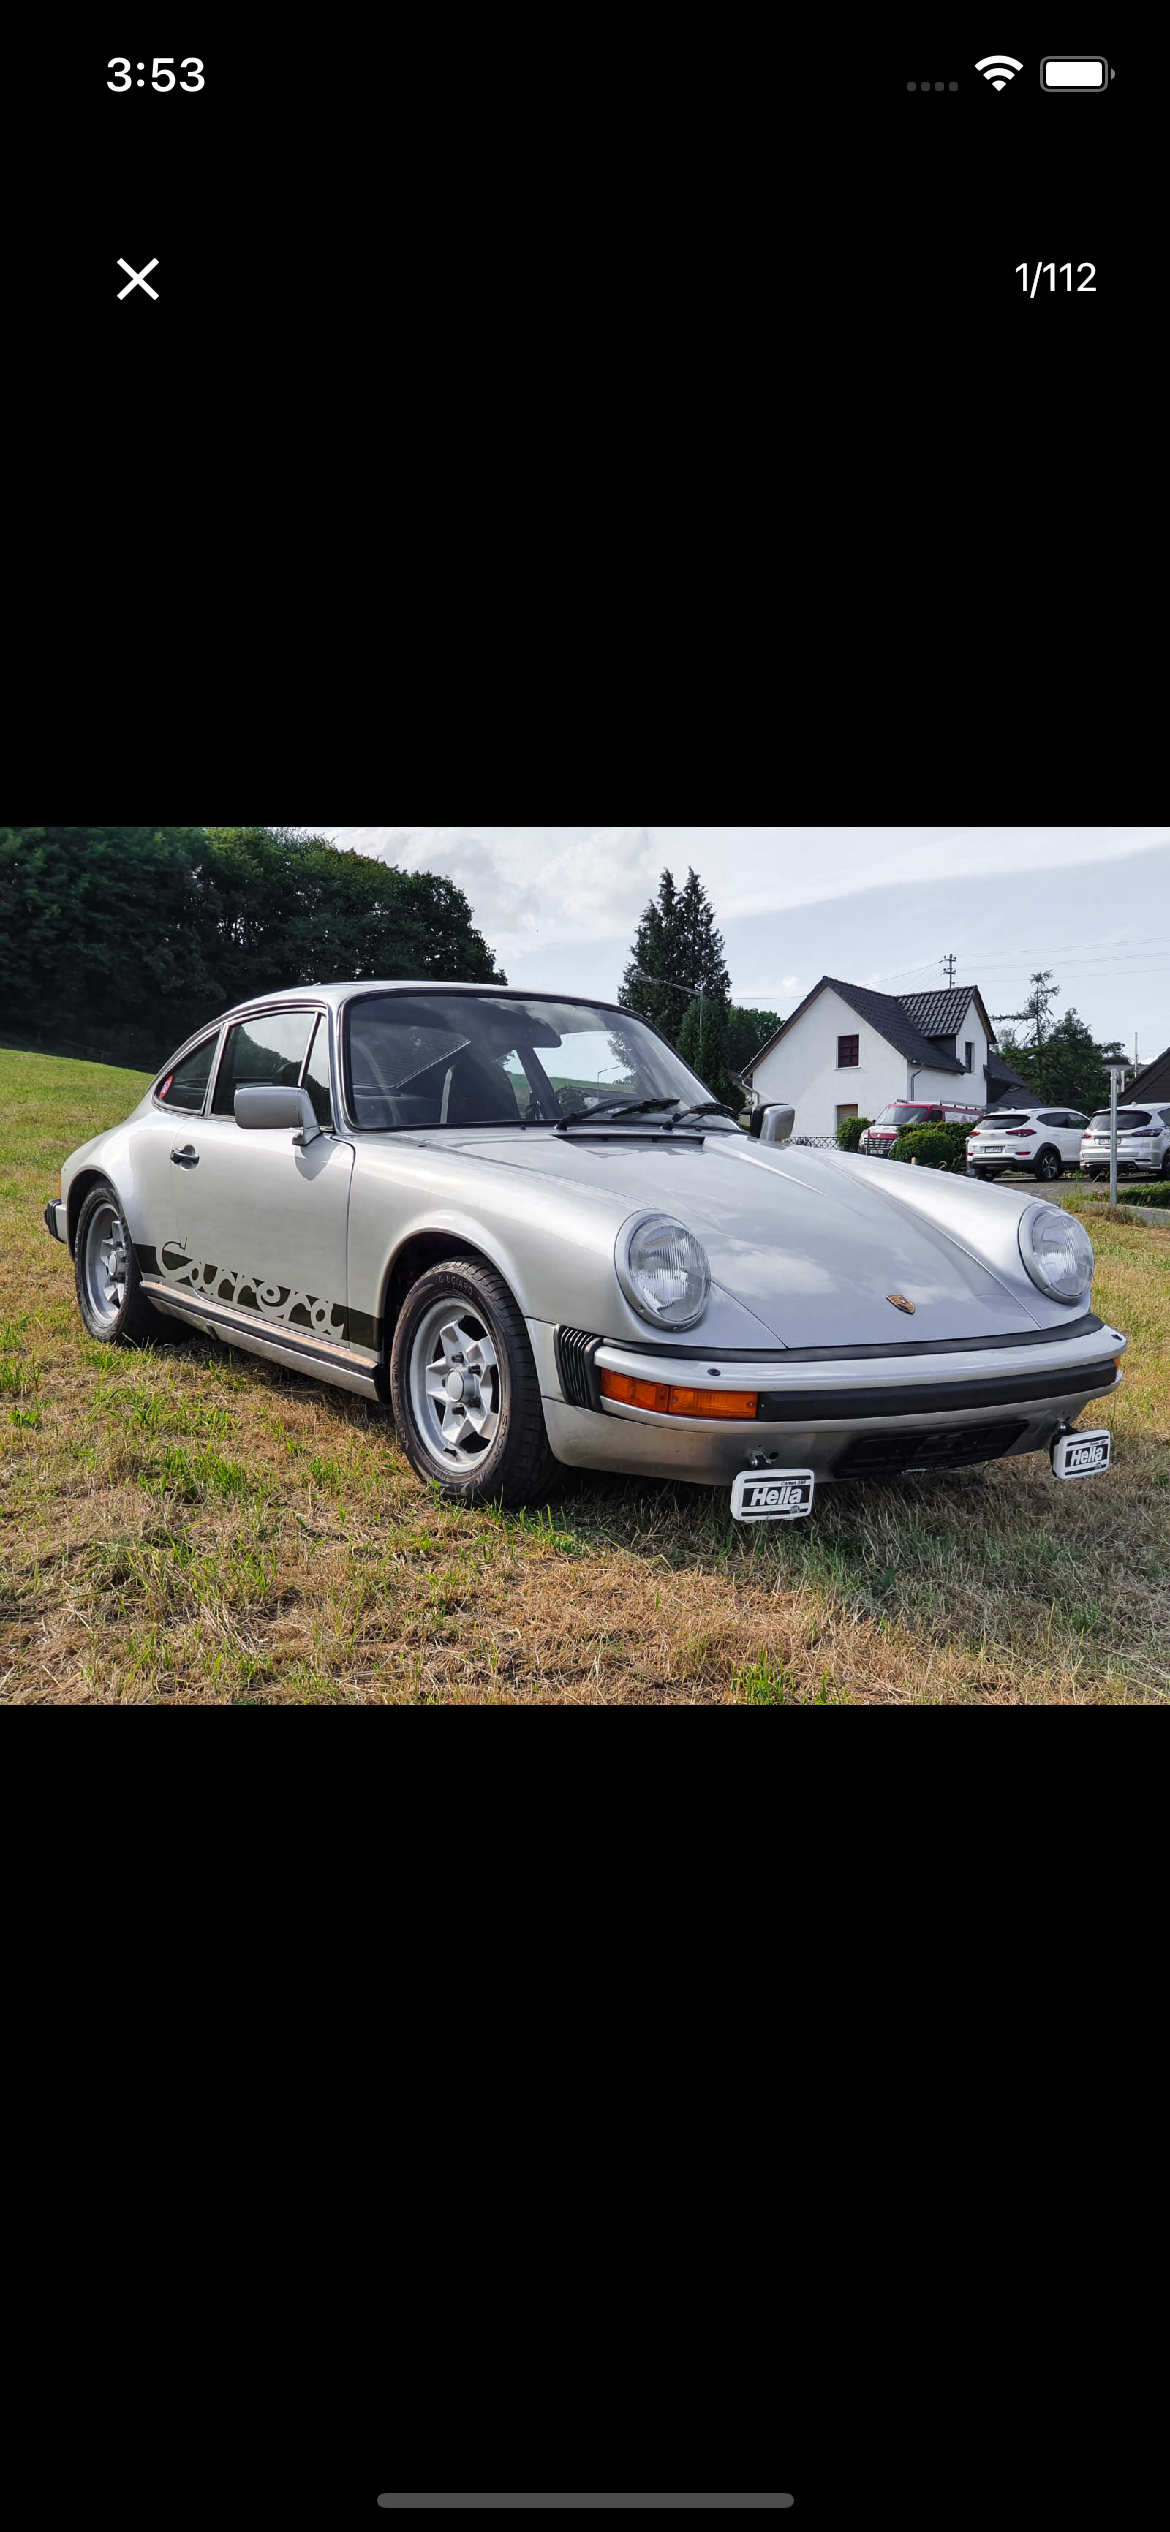
\includegraphics[width=\linewidth, height=300pt]{images/kickdown_presentation/kickdown_gallery.png}}
            \caption{Kickdown Gallery View}
            \label{fig:kickdown_gallery_view}
        \end{minipage}
        &
        \begin{minipage}{.33\textwidth}
            \centering
            \fbox{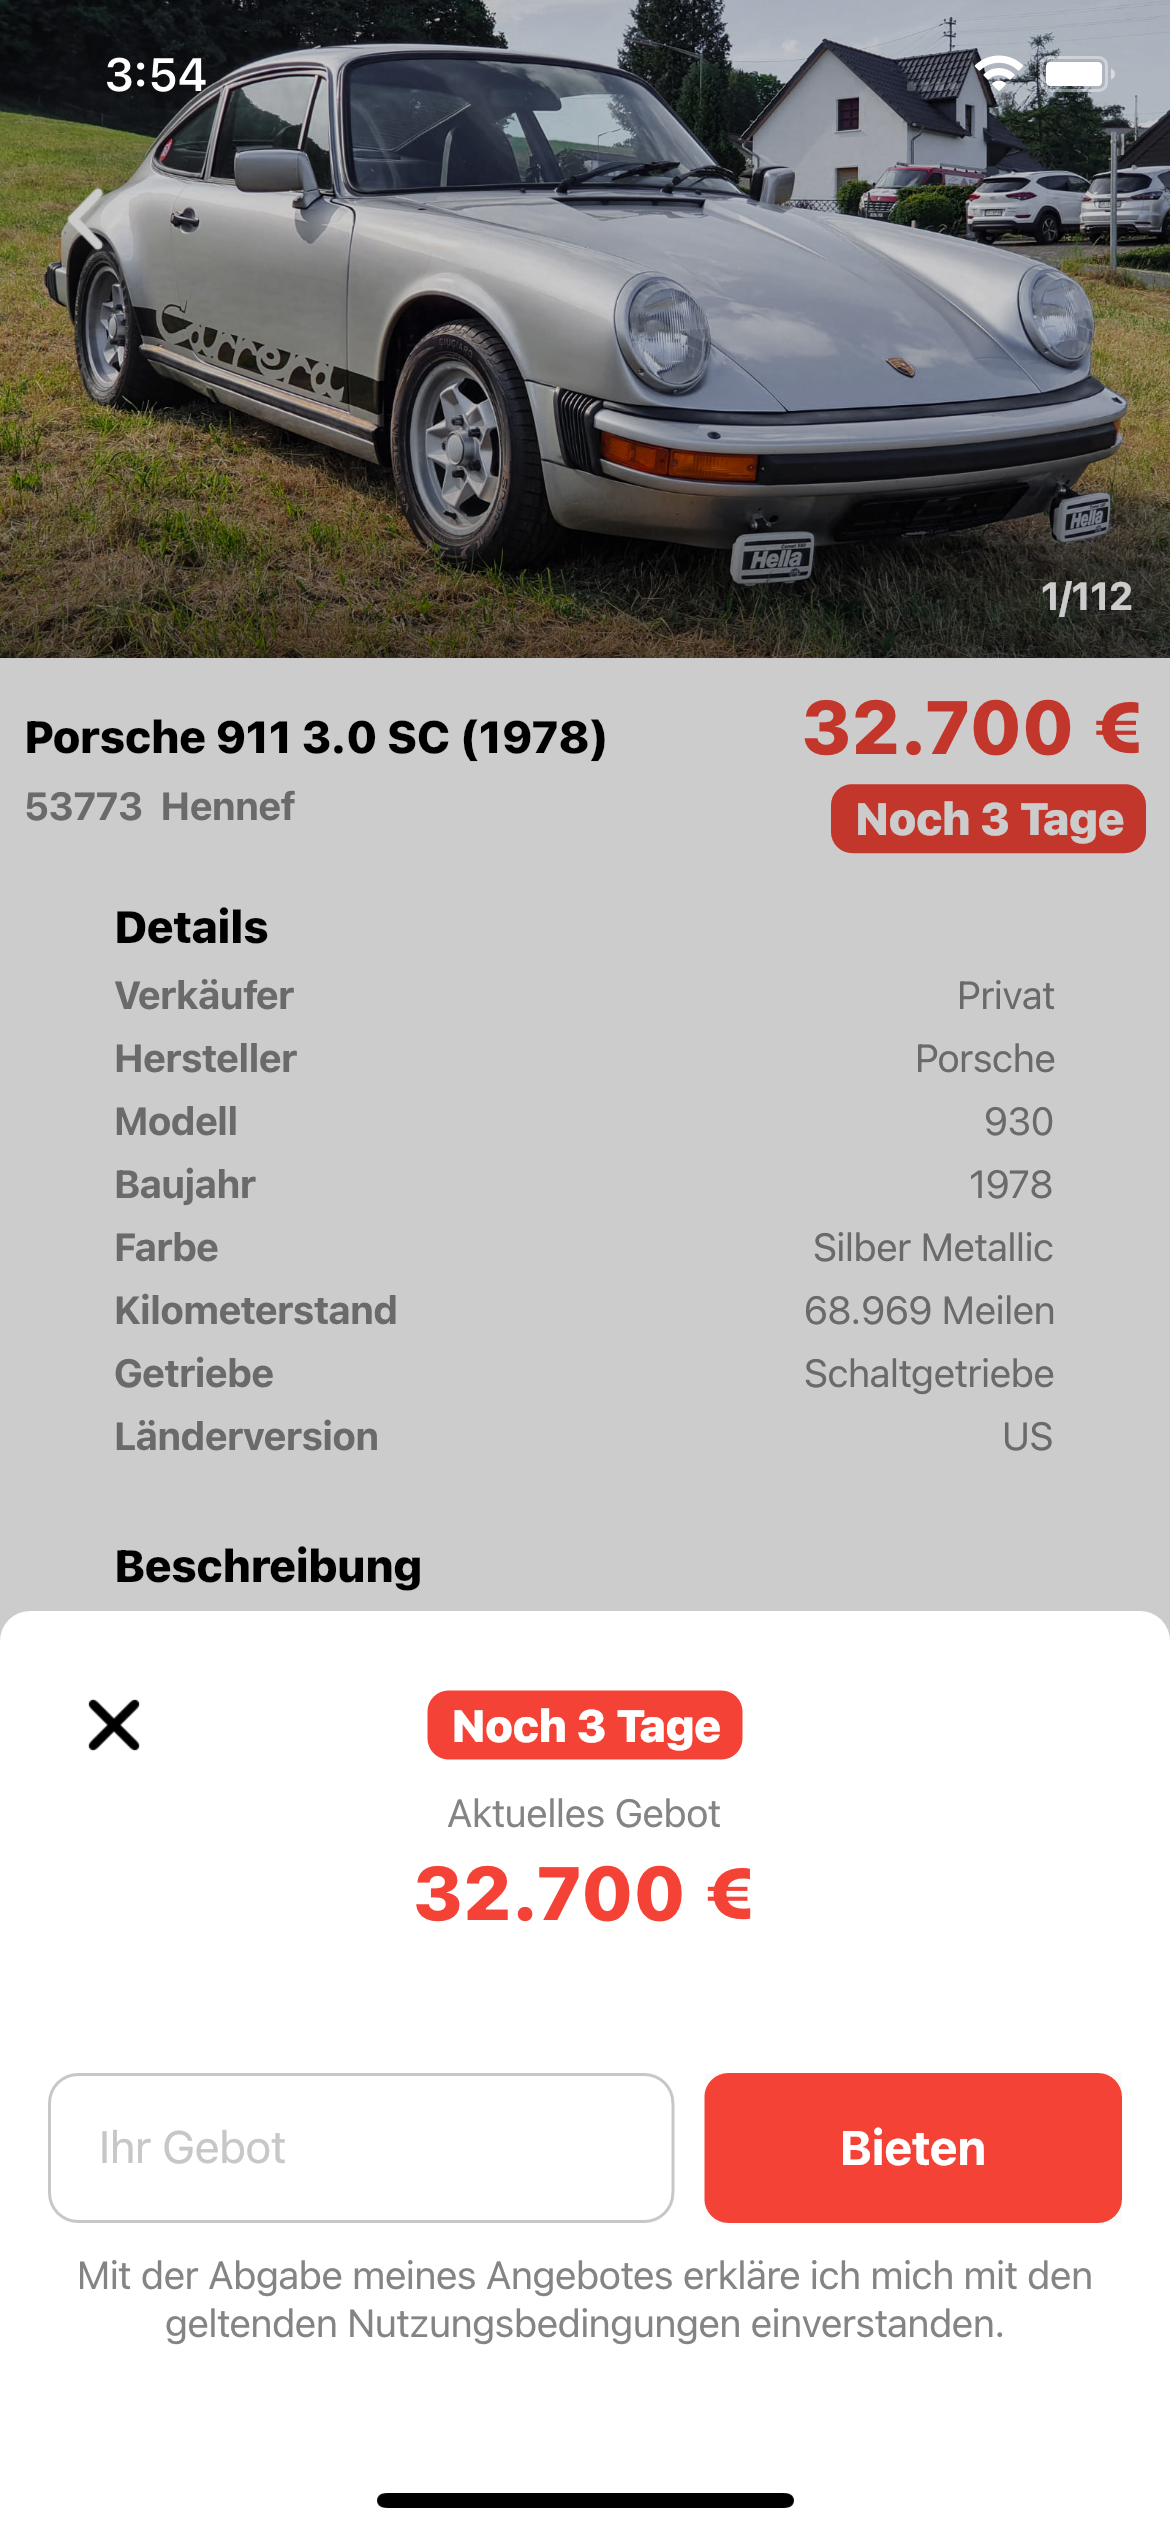
\includegraphics[width=\linewidth, height=300pt]{images/kickdown_presentation/kickdown_bid_preparation_screen.png}}
            \caption{Kickdown Bid Preparation Screen}
            \label{fig:kickdown_bid_preparation_screen}
        \end{minipage}
    \end{tabular}
\end{figure}

\section{Performance Comparison} \label{section::performance_comparison_design}
The methodology chosen to empirically test the performance hypthesis $H_P$ (Section \ref{section::thesis_objective}) is a quantitative
measurement of computational resources during app runtime. Measurements are performed for
specific load conditions (i.e use cases). In the process, the original app acts as an empirical
baseline for testing the Flutter replica against.\\
Directly benchmarking system resources provides insight whether the Flutter framework consumes
compute resources efficiently under typically imposed load settings. Furthermore, system
benchmarking metrics are the underlying cause of more ephemeral measures for testing the
system load itself, e.g. page load time. In addition, the chosen compute resources (explained
in Section \ref{subsection::selected_measurement_variables}) are easily measured using software tooling (Section \ref{subsection::profiling_tooling}) which aids the
objectivity, reliability and validity of this particular study methodology.
Finally, the data is statistically evaluated in order to make inferences about the hypothesis.

\subsection{Selected Performance Measurement Variables} \label{subsection::selected_measurement_variables}
The following paragraphs introduce the selected performance measurement variables. Concretely,
a brief definition is given as well as the reasoning for including the particular metric in
this study with regards to evalutating the performance hypothesis (Section \ref{section::thesis_objective}).

\paragraph*{CPU Utilization}\label{paragraph::cpu_utilization}\hfill \break
CPU utilization is defined as the CPU time (\cite{FSF1988}) of a task
divided by its overall capacity expressed as a percentage. 
The CPU is partly responsible for rendering related calculations.
For example, Flutter's tree diffing algorithm is handled on the CPU.
Therefore, testing CPU utilization assesses whether Flutter's framework processing requirements for rendering related calculations can be fulfilled on the testing hardware (Section \ref{subsection::measurement_process}).

\paragraph*{GPU Utilization}\label{paragraph::fps}\hfill \break
GPU utilization is the GPU equivalent of CPU utilization mentioned in \ref{paragraph::cpu_utilization}.
The GPU is a specialized processing chip optimized graphics computation.
The CPU and GPU are tightly integrated on iPhones which make use of the System-on-a-Chip architecture (\cite{Martin2001}, \cite{WikiChip2020}).
Therefore a strong correspondence between CPU and GPU usage should be observed in the study. 
Nonetheless, testing GPU utilization by itself is a valuable metric for determining Flutter's graphic specific processing needs.

\paragraph*{Memory Utilization}\label{paragraph::memory_utilization}\hfill \break
Memory utilization is the percentage of available memory capacity used for a specific task. 
A high level of memory usage negatively impacts performance of running tasks as well as interactive responsiveness (\cite{Ljubuncic2015}).

\subsection{Measurment Process} \label{subsection::measurement_process}
To reduce measurement confounders, the device is restarted before each individual measurement to ensure that all
irrelevant background processes are cancelled.\\
The measurement process for the individual metrics is further split into specific user actions
which are executed and tested on both the iOS and Flutter app separately. These were chosen
to test all relevant facets of the app (see Section \ref{section:kickdown_feature_presentation}) and ensure a sufficient load on the system:
\begin{itemize}
    \item \textbf{app start:} The app is freshly installed on the test device, opened and idle until the visible postings are loaded.
    \item \textbf{scrolling:} On the postings overview screen, the posting cards are vertically scrolled fully to the bottom and subsequently back to the top.
    \item \textbf{detail view:} From the postings overview, the first posting is tapped to navigate to the detail view. Afterwards the back button is tapped to navigate back to the overview.
    \item \textbf{image gallery:} The image gallery of a posting is opened from the detail view of a posting and the first 10 images are viewed by swiping.
\end{itemize}
For each \textbf{user action}, the average of all values over time is recorded. This process is then
repeated 3 times and averaged. The exact number of experiment repetitions was chosen as a
tradeoff between marginal accuracy increase and additional experiment execution time.\\
Furthermore, 2 testing rounds are devised on separate devices. The iPhone 12 Pro and iPhone
6s are chosen as the upper and lower bounds of hardware performance respectively. The lower
bound is defined in this case as per Apples recommendation to set the deployment target to the
current operating system version (iOS 14 at time of writing) minus one (iOS 13) which lists the
iPhone 6s as the oldest supported device (\cite{Apple2021}). iOS 13 is also the minimum deployment target for the Kickdown app.\\

\subsection{Profiling Tools} \label{subsection::profiling_tooling}
\textbf{Xcode Instruments} (\cite{Apple2019}) - a part of the \textbf{Xcode} IDE tool set - are used for profiling the individual metrics. It provides multiple preconfigured
profiling trace instruments.
For the purposes of this thesis, the \textbf{Time Profiler} tool (see Figure \ref{fig:time_profiler_graph} and \ref{fig:time_profiler_table}) is used for CPU (see Paragraph \ref{paragraph::cpu_utilization}),
the \textbf{Allocations} tool (see Figure \ref{fig:allocations_profiler_graph} and \ref{fig:allocations_profiler_table}) for memory usage (see Paragraph \ref{paragraph::memory_utilization}) and \textbf{Core Animation} tool (see Figure \ref{fig:core_animation_profiler_graph} and \ref{fig:core_animation_profiler_table}) for FPS (see Paragraph \ref{paragraph::fps}).
For each profiling tool a graph shows the particular metric quantified over time with an associated table showing the exact numeric values with time stamps.

\begin{figure}[htbp]
    \begin{tabular}{p{0.5\textwidth}p{0.5\textwidth}}
        \begin{minipage}{.5\textwidth}
        \centering
        \includegraphics[width=\linewidth]{images/profiling/time_profiler/time_profiler_graph.eps}
        \caption{Time Profiler Graph}
        \label{fig:time_profiler_graph}
        \end{minipage}
        &
        \begin{minipage}{.5\textwidth}
            \centering
            \includegraphics[width=\linewidth]{images/profiling/time_profiler/time_profiler_table.eps}
            \caption{Time Profiler Table}
            \label{fig:time_profiler_table}
        \end{minipage}
    \end{tabular}
\end{figure}

\begin{figure}[htbp]
    \begin{tabular}{p{0.5\textwidth}p{0.5\textwidth}}
        \begin{minipage}{.5\textwidth}
        \centering
        \includegraphics[width=\linewidth]{images/profiling/allocations_profiler/allocations_graph.eps}
        \caption{Allocations Profiler Graph}
        \label{fig:allocations_profiler_graph}
        \end{minipage}
        &
        \begin{minipage}{.5\textwidth}
            \centering
            \includegraphics[width=\linewidth]{images/profiling/allocations_profiler/allocations_table.eps}
            \caption{Allocations Profiler Table}
            \label{fig:allocations_profiler_table}
        \end{minipage}
    \end{tabular}
\end{figure}

\begin{figure}[htbp]
    \begin{tabular}{p{0.5\textwidth}p{0.5\textwidth}}
        \begin{minipage}{.5\textwidth}
        \centering
        \includegraphics[width=\linewidth]{images/profiling/core_animation/core_animation_graph.eps}
        \caption{Core Animation Profiler Graph}
        \label{fig:core_animation_profiler_graph}
        \end{minipage}
        &
        \begin{minipage}{.5\textwidth}
            \centering
            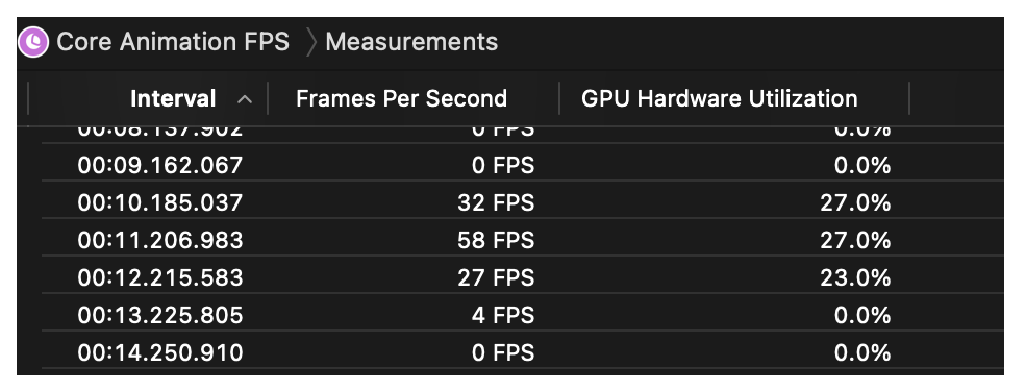
\includegraphics[width=\linewidth]{images/profiling/core_animation/core_animation_table.eps}
            \caption{Core Animation Profiler Table}
            \label{fig:core_animation_profiler_table}
        \end{minipage}
    \end{tabular}
\end{figure}



\subsection{Evaluation Process} \label{subsection::evaluation_process}
To better understand the data gathered, it is subsequently examined using exploratory data
analysis (EDA) (\cite{Tukey1977}).


\section{User Experience Comparison} \label{section::usability_comparison_design}
%%% Goal %%%
This Section explores the usability hypothesis evaluation methodology. Specifically, laying out
the procedure to answer the question of whether or not the Flutter framework is capable of
reproducing native iOS application user experiences (see Section \ref{section::thesis_objective}).

%%% Problem with measuring UX and why performance results are used %%%
Generally, as UX is built for other humans, any evaluation is prone to subjectivity and perception
biases (\cite{Tversky1974}). Therefore, it is difficult to capture these impressions quantitatively in a reproducable manner.\\
However, the user experience of an app is directly dependant upon sufficiently underlying performance (e.g. for scrolling
fluidity). Therefore the results of the performance comparison (Section \ref{section::performance_comparison}) form the basis of the evaluation of the usability hypothesis $H_U$.
Utilizing a mixed approach as a study methodology combining both the quantitative performance comparison and a qualitative method will draw upon the strengths of both approaches. 

%%% Why I'm using expert interviews %%%
Specifically, \textit{semi structured interviews with subject matter experts} (see \cite{Liebold2009}) are conducted to evaluate the baseline application
with the Flutter replica by asking the participants for differences between the two apps (further explained in Section \ref{subsection::interview_guideline}). This methodology has the
advantage of covering predetermined topics relevant to the research question while also allowing spontaneous discussion possibly leading to novel insights.\\
Furthermore, expert interviews are an especially useful approach for scientific explorations
with no or scant preexisting theory (see \cite{Experts2009}).

%%% Number of interviews conducted %%%
As soon as no new perspectives seem to emerge during interviews, no further interviews will be conducted.
This is based on the fact that the method of expert interviews 
aims to provide a breadth of perspectives on a given topic unlike specific quantitative anaylses (see \cite{Liebold2009}).


\subsection{Interview Preliminaries and Technicalities}
The interviews are conducted with employees of apploft. They qualify as subject matter experts in the sense that they have been working in the mobile app industry for multiple years. They come from a variety
of professional backgrounds including UX and UI design, project management as well as software engineering. Furthermore, some interviewees have actually worked on the original app itself. This diversity 
among the study participants is especially relevant in order to explore a breadth of perspectives. 
Due to the ongoing Covid-19 pandemic, the interviews are conducted through video calls, are recoreded with the interviewees consent and the interviewees are asked to share their iPhone screen via Quicktime player (\cite{Apple2014}).
The moderation and recording is facilitated by the author.
For the comparison, the interviewees receive QR codes with which both apps may be downloaded. Behind each distributed code is a downloadable IPA (iOS App Store Package) binary executable file hosted by an HTTP server.
These work exactly the same as any other apps downloaded from the iOS App Store.
Both apps are blindly distributed to the participants as "Kickdown A" and "Kickdown B" in order to remove confirmation bias as a confounder (see \cite{Tversky1974}).

\subsection{Interview Guideline} \label{subsection::interview_guideline}
%% Goal %%%
The interview guideline (see Appendix \ref{section::interview_guideline}) is based on finding out perceptual differences between the iOS baseline and Flutter replica app.

%% Use Cases %%
Just like the performance comparison, use cases associated with particular UI facets form the basis for the evaluation:
\begin{itemize}
    \item \textbf{App Start and Scroll Behavior}
    \item \textbf{Detail Transition, Modal Transition, Textfield interaction}
    \item \textbf{Horizontal Scrolling}
    \item \textbf{Switch Interaction}
\end{itemize}
The interviewees are asked to perform a particular use case for app A and app B. Then they are asked to detail differences between the two apps.
Asking this open-ended question aims at receiving as much information possible about perceptual differences (Cf. \cite[182--185]{Helferrich2011}).
Subsequently, the participant is asked to determine which of the two apps felt more natural (i.e. had a better UX). A determined trivalent response of: "A", "B" or "same" is expected. 
The goal of this question is to get overall impression of the usability. \\
Both questions are asked after each use case execution of the participant. 
To maintain a high participant engagement during interviews, use cases are described in a more captivating way, e.g. "Please find the blue Mercedes SUV in Kickdown A [Wait until participant has found it.]. Now, 
please look for the black BMW convertible in the other app.". 
After each use case, the ordering of app A and B is swapped. E.g. if the first case starts with A, the second starts with B. This choice is made as to avoid recency bias (Cf. \cite{Atkinson1968}).
Furthermore, the ordering is also swapped after each interview. In this way, participant X starts with app A while participant Y starts with B.
Finally, after the last use case, the participant is asked to answer the two questions with regard to the entire application.


\subsection{Interview Evaluation} \label{section::interview_evaluation}
The videos from the interviews are transcribed into a textual format and further processed using \textbf{interview coding}. Thereby, each interview is categorized into semantic themes. These themes among
all interviews are then merged into an overall theme structure - also known as code structure. This code structure forms the basis for the evaluation of the usability hypothesis $H_U$. 
% Todo: Further research this topic.